\chapter{RESULTS AND DISCUSSION}
This chapter describes the implementation and results of the empirical analysis
outlined above.  Each section of this chapter details one of the three main
tasks of the empirical analysis.  The first task is to create synthetic data,
the second to train the SOMs and finally to apply the diagnostics.

\section{Data}
%The data will be generated with the common technique of rejection sampling,
%where n high dimensional seeds are chosen at random, samples will be taken
%at random from a uniform distribution, if the sample falls with in radius r of
%any seed it is accepted, if it does not, single random number is drawn, if that
%number is \(<\) 0.05\% the sample is accepted as noise, else the sample is rejected.
The training data will be generated using a Gaussian cluster generator as
described by \cite{handl}.  To generate the data we have to decide how many
clusters to create and how many dimensions to use.  In order to set these
parameters appropriately we will first explore how the internal variance
responds to adjustments in their value.

To accomplish this twenty test datasets are generated and used to train each
topology, for a total of eighty SOMs. Table \ref{ivtable1} shows the average
internal variance of each SOM.  All topologies seem to respond similarly. The
internal variance of the SOM increases as we add dimensions and decreases as
we add clusters. Based on these results, it was decided that five dimensions
and ten clusters was a reasonable choice. Five dimensions is easier to work
with than larger numbers and should yield more information than two
dimensions. Ten clusters was chosen because, the internal variances seemed to
level out near this number.

The results shown in table \ref{ivtable1} are in line with what one would
expect.  The SOM has a hard time organizing the random datasets (the datasets
with no clusters are just random data) resulting more competition between
neurons and higher internal variances. It has a much easier time organizing
data with some kind of structure (i.e. clusters).  Somewhat surprising
however, is how similar the results are between topology types.  We'll examine
this in more detail later.  In the future it may be of interest to look at how the
internal variance responds to uniformly distributed data.
% it would be interesting to try unformly distiburted data here, the SOM could
% be used to decide if your data is clustered, uniform or random.

\begin{table}
\caption{Mean Internal Variance}
\label{ivtable1}
\centering

\subtable[Rook Topology]{
  \begin{tabular}{|c||c|c|c|c|}
  \hline
  &\multicolumn{4}{c|}{\textbf{Dimensions}}\\
  \textbf{Clusters} & \multicolumn{1}{c}{\textbf{2}} &
  \multicolumn{1}{c}{\textbf{5}} & \multicolumn{1}{c}{\textbf{10}} &
  \multicolumn{1}{c|}{\textbf{20}}\\
  \hline
  \hline
  \textbf{0} & 0.0206& 0.2776& 0.7299& 1.4168 \\
  \hline
  \textbf{2} & 0.0112& 0.1095& 0.2687& 0.4829 \\
  \hline
  \textbf{5} & 0.0108& 0.0961& 0.2260& 0.4281 \\
  \hline
  \textbf{10} & 0.0113& 0.0914& 0.2055& 0.4129 \\
  \hline
  \textbf{20} & 0.0112& 0.0868& 0.2004& 0.3970 \\
  \hline
  \end{tabular}
  \label{ivtable:rook}
}
\subtable[Hexagonal Topology]{
  \begin{tabular}{|c||c|c|c|c|}
  \hline
  &\multicolumn{4}{c|}{\textbf{Dimensions}}\\
  \textbf{Clusters} & \multicolumn{1}{c}{\textbf{2}} &
  \multicolumn{1}{c}{\textbf{5}} & \multicolumn{1}{c}{\textbf{10}} &
  \multicolumn{1}{c|}{\textbf{20}}\\
  \hline
  \hline
  \textbf{0} & 0.0205& 0.2786& 0.7295& 1.4189 \\
  \hline
  \textbf{2} & 0.0109& 0.1108& 0.2683& 0.4813 \\
  \hline
  \textbf{5} & 0.0101& 0.0960& 0.2243& 0.4269 \\
  \hline
  \textbf{10} & 0.0108& 0.0902& 0.2049& 0.4128 \\
  \hline
  \textbf{20} & 0.0112& 0.0861& 0.2019& 0.3969 \\
  \hline
  \end{tabular}
  \label{ivtable1:hex}
}
\subtable[Spherical Topology]{
  \begin{tabular}{|c||c|c|c|c|}
  \hline
  &\multicolumn{4}{c|}{\textbf{Dimensions}}\\
  \textbf{Clusters} & \multicolumn{1}{c}{\textbf{2}} &
  \multicolumn{1}{c}{\textbf{5}} & \multicolumn{1}{c}{\textbf{10}} &
  \multicolumn{1}{c|}{\textbf{20}}\\
  \hline
  \hline
  \textbf{0} & 0.0207& 0.2650& 0.7124& 1.3983 \\
  \hline
  \textbf{2} & 0.0108& 0.1079& 0.2644& 0.4768 \\
  \hline
  \textbf{5} & 0.0104& 0.0950& 0.2231& 0.4213 \\
  \hline
  \textbf{10} & 0.0110& 0.0888& 0.2040& 0.4105 \\
  \hline
  \textbf{20} & 0.0117& 0.0841& 0.2007& 0.3953 \\
  \hline
  \end{tabular} 
  \label{ivtable1:graph}
} 
\subtable[Geodesic Sphere Topology]{
  \begin{tabular}{|c||c|c|c|c|}
  \hline
  &\multicolumn{4}{c|}{\textbf{Dimmensions}}\\
  \textbf{Clusters} & \multicolumn{1}{c}{\textbf{2}} &
  \multicolumn{1}{c}{\textbf{5}} & \multicolumn{1}{c}{\textbf{10}} &
  \multicolumn{1}{c|}{\textbf{20}}\\
  \hline
  \hline
  \textbf{0} & 0.0208& 0.2659& 0.7135& 1.3983 \\
  \hline
  \textbf{2} & 0.0108& 0.1068& 0.2641& 0.4778 \\
  \hline
  \textbf{5} & 0.0105& 0.0945& 0.2226& 0.4222 \\
  \hline
  \textbf{10} & 0.0111& 0.0871& 0.2032& 0.4108 \\
  \hline
  \textbf{20} & 0.0117& 0.0849& 0.1993& 0.3945 \\
  \hline
  \end{tabular}
  \label{ivtable1:geodesic}
}
\end{table}

\section{Training}
Before we can go on to addressing the research questions we need to train a
series of SOMs. One problem that we will face is a small group size when the
neurons of a given SOM are grouped by their degree.  For example in the rook
topology there are only four neurons that have a degree of two, the four
corners. The rest of the neurons have three or four neighbors depending on
whether they are on the edge or not. To deal with this problem we will try to
increase the sample size by combining the results of many SOMs trained with
similar data.

The four topologies are tested. These are the Rook, Hexagonal, Geodesic Sphere
and a forth topology based on a \cite{Rakhmanov94}. As mentioned before
\cite{Rakhmanov94} suggest a method for distributing an arbitrary number of
point on to the surface of a sphere.  Delaunay triangulation is applied to the
result of this method producing a topological structure for the points.  This
topology shall be is referred to simply as ``spherical.''  As shown in figure
\ref{fig:nSize} the achievable network size is rather limited in the geodesic
SOM.  An eight frequency geodesic sphere has 642 nodes. The hexagon and rook
topologies can achieve 644 nodes when the dimensions set to 28 by 23. The
spherical topology will be set to 642 nodes.

Ten synthetic datasets are generated using the parameters described in the
previous section. The datasets are used to train SOMs for each topology
resulting in another forty SOMs. The average internal variance of these SOMs
are summarized in Table \ref{ivtable3}.  We find that the mean internal
variance seems to remain fairly stable, this suggests that we can combine the
results of each simulation within a given topology. In the rook topology we
will now have up to forty\footnote{We can only measure the internal variance
when a neuron captures two or more observations from the training data.
Therefore, it would be possible to have less than forty measurements.}
internal variance measurements for neurons with only two neighbors.

\begin{table}[hbt]
\centering
\caption{Mean IV for each simulation, by topology}
\label{ivtable3}
\begin{tabular}{|c||c|c|c|c|}
\hline
\textbf{Simulation Number} & Geodesic & Spherical & Hex & Rook \\
\hline
\hline
\textbf{1} & 0.0871 & 0.0888 & 0.0902 & 0.0914 \\
\hline
\textbf{2} & 0.0873 & 0.0877 & 0.0871 & 0.0879 \\
\hline
\textbf{3} & 0.0772 & 0.0782 & 0.0781 & 0.0779 \\
\hline
\textbf{4} & 0.0897 & 0.0889 & 0.0876 & 0.0912 \\
\hline
\textbf{5} & 0.0864 & 0.0876 & 0.0875 & 0.0866 \\
\hline
\textbf{6} & 0.0826 & 0.0839 & 0.0859 & 0.0851 \\
\hline
\textbf{7} & 0.0902 & 0.0905 & 0.0921 & 0.0920 \\
\hline
\textbf{8} & 0.1001 & 0.1000 & 0.1005 & 0.0999 \\
\hline
\textbf{9} & 0.0805 & 0.0807 & 0.0818 & 0.0827 \\
\hline
\textbf{10} & 0.0929 & 0.0925 & 0.0937 & 0.0951 \\
\hline
\end{tabular} \end{table}

\section{Diagnostics}
This section applies the our three diagnositcs to the SOMs that were trained
above.  All three build on the idea of an internal variance \(I_v\), defined
for neuron \(i\) as the 

 \begin{equation}
\frac{2}{n^2-n}\sum_{j=1}^n\sum_{k=1}^n ||x_{ij}-x_{ik}||
 \label{eqno1}
 \end{equation}

The first looks at how internal variance changes with a neuron's first
order neighborhood size, or degree.  The second.


\subsection{Internal variance vs. first-order neighborhood size}
After the internal variance and degree of each neuron are calculated we
group the neurons for a given topology by their degree. The number for groups
we end up with varies by topology. Figure \ref{boxplot} offers a visualization
of these groups for each topology.  Each sub-figure shows a series of box
plots, each representing the distribution of internal variance within a given
group.  It was originally expected that the internal variances would be lower
for groups with larger degrees. This figure suggests that is only true for the
``flat'' topologies.

\begin{figure}[hbt]
\label{boxplot}
\centering
\subfigure[Rook Topology]{
  \label{boxplot:rook}
  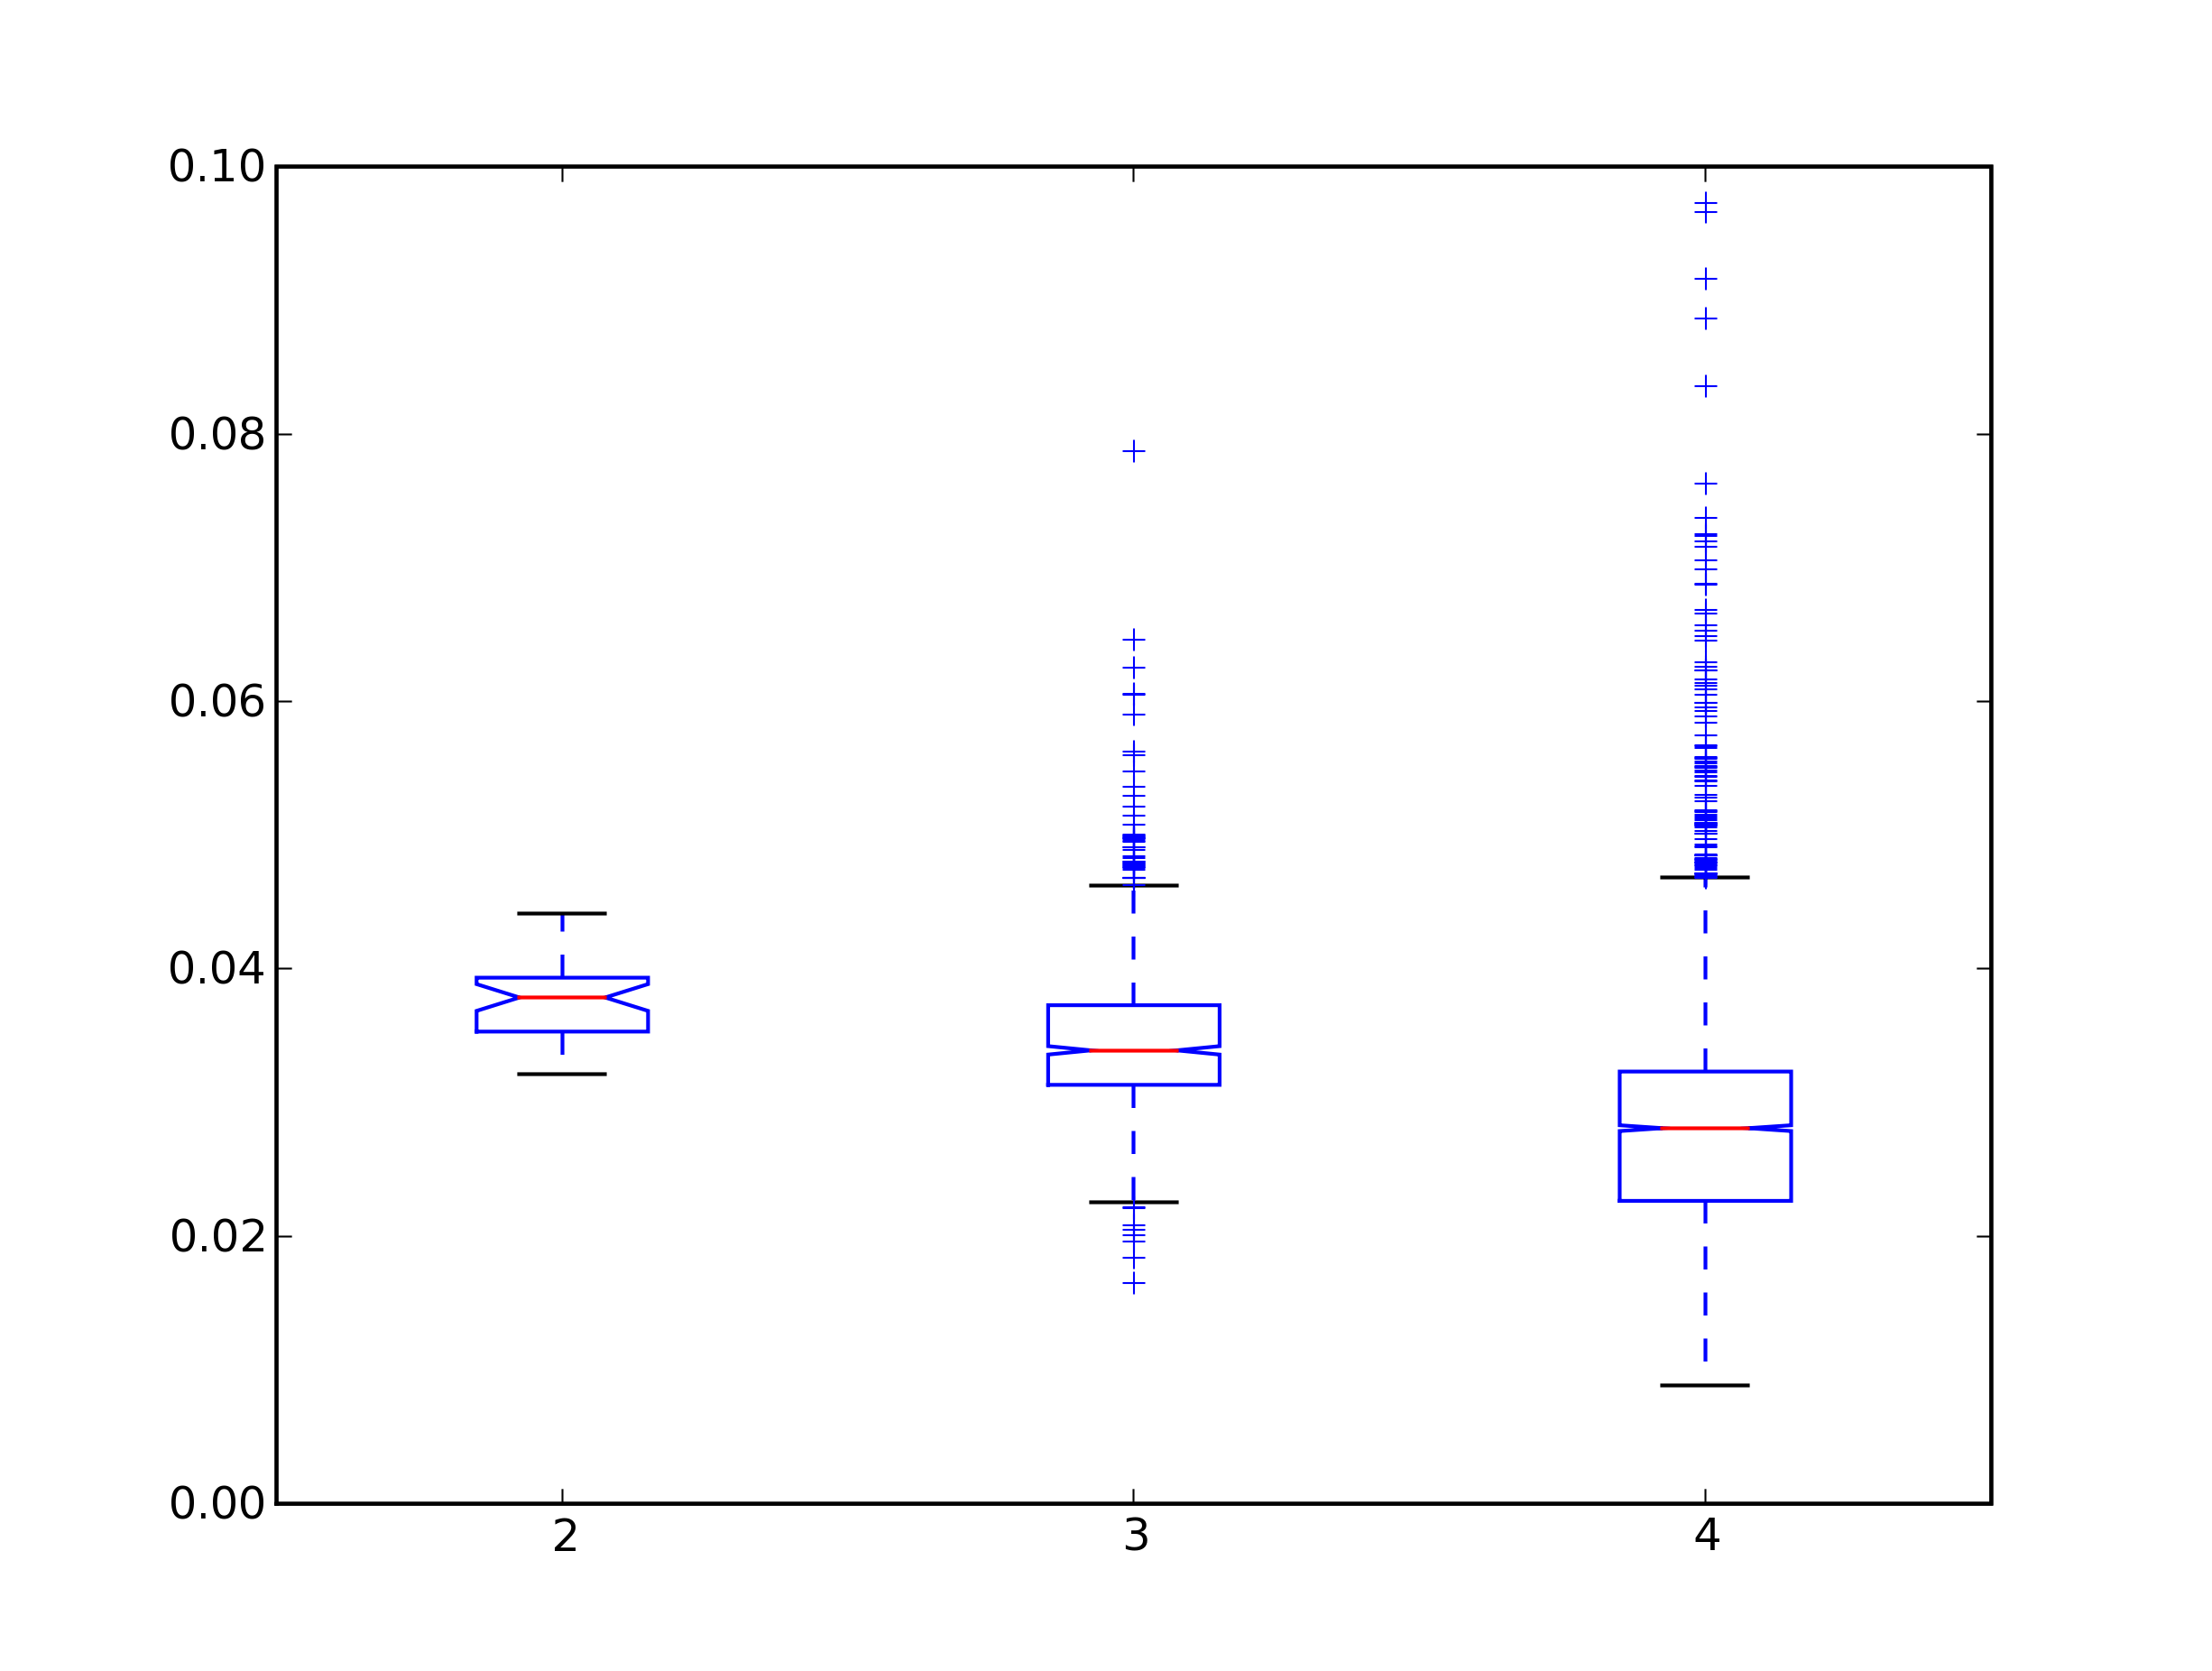
\includegraphics[width=.45\linewidth]{rook_iv_box.png}
}
\subfigure[Hexagonal Topology]{
  \label{boxplot:hex}
  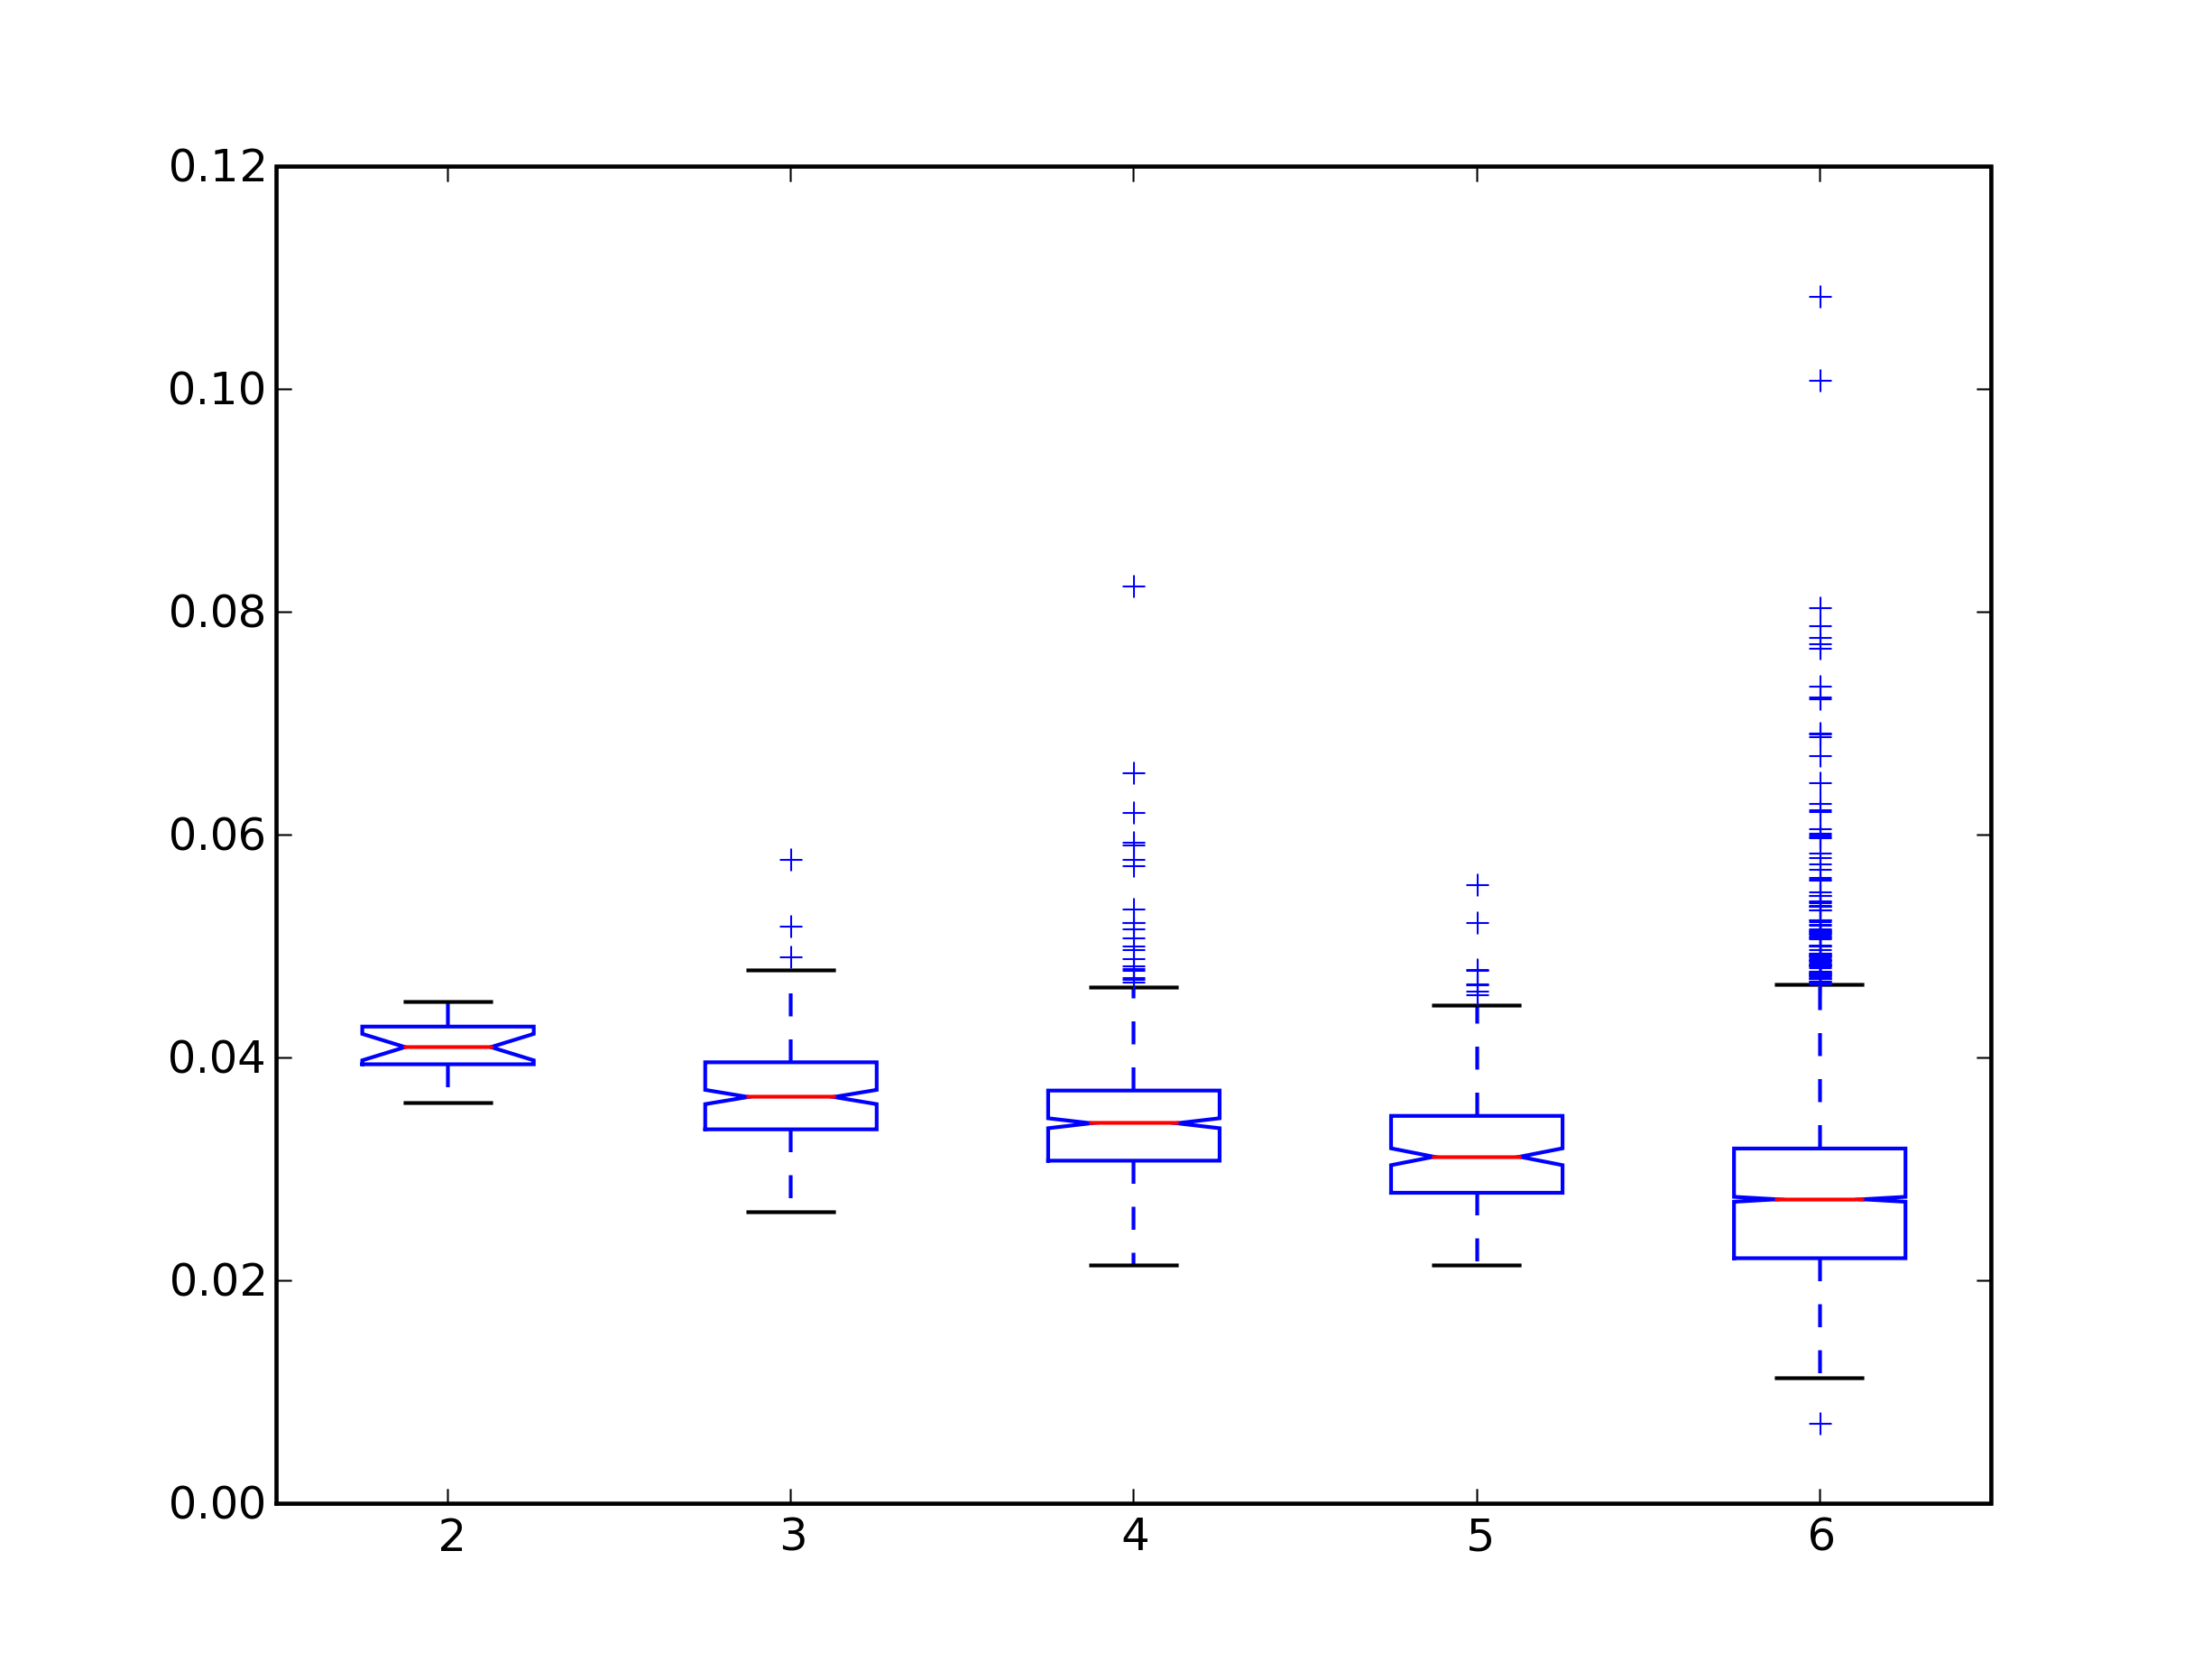
\includegraphics[width=.45\linewidth]{hex_iv_box.png}
}
\subfigure[Spherical Topology]{
  \label{boxplot:graph}
  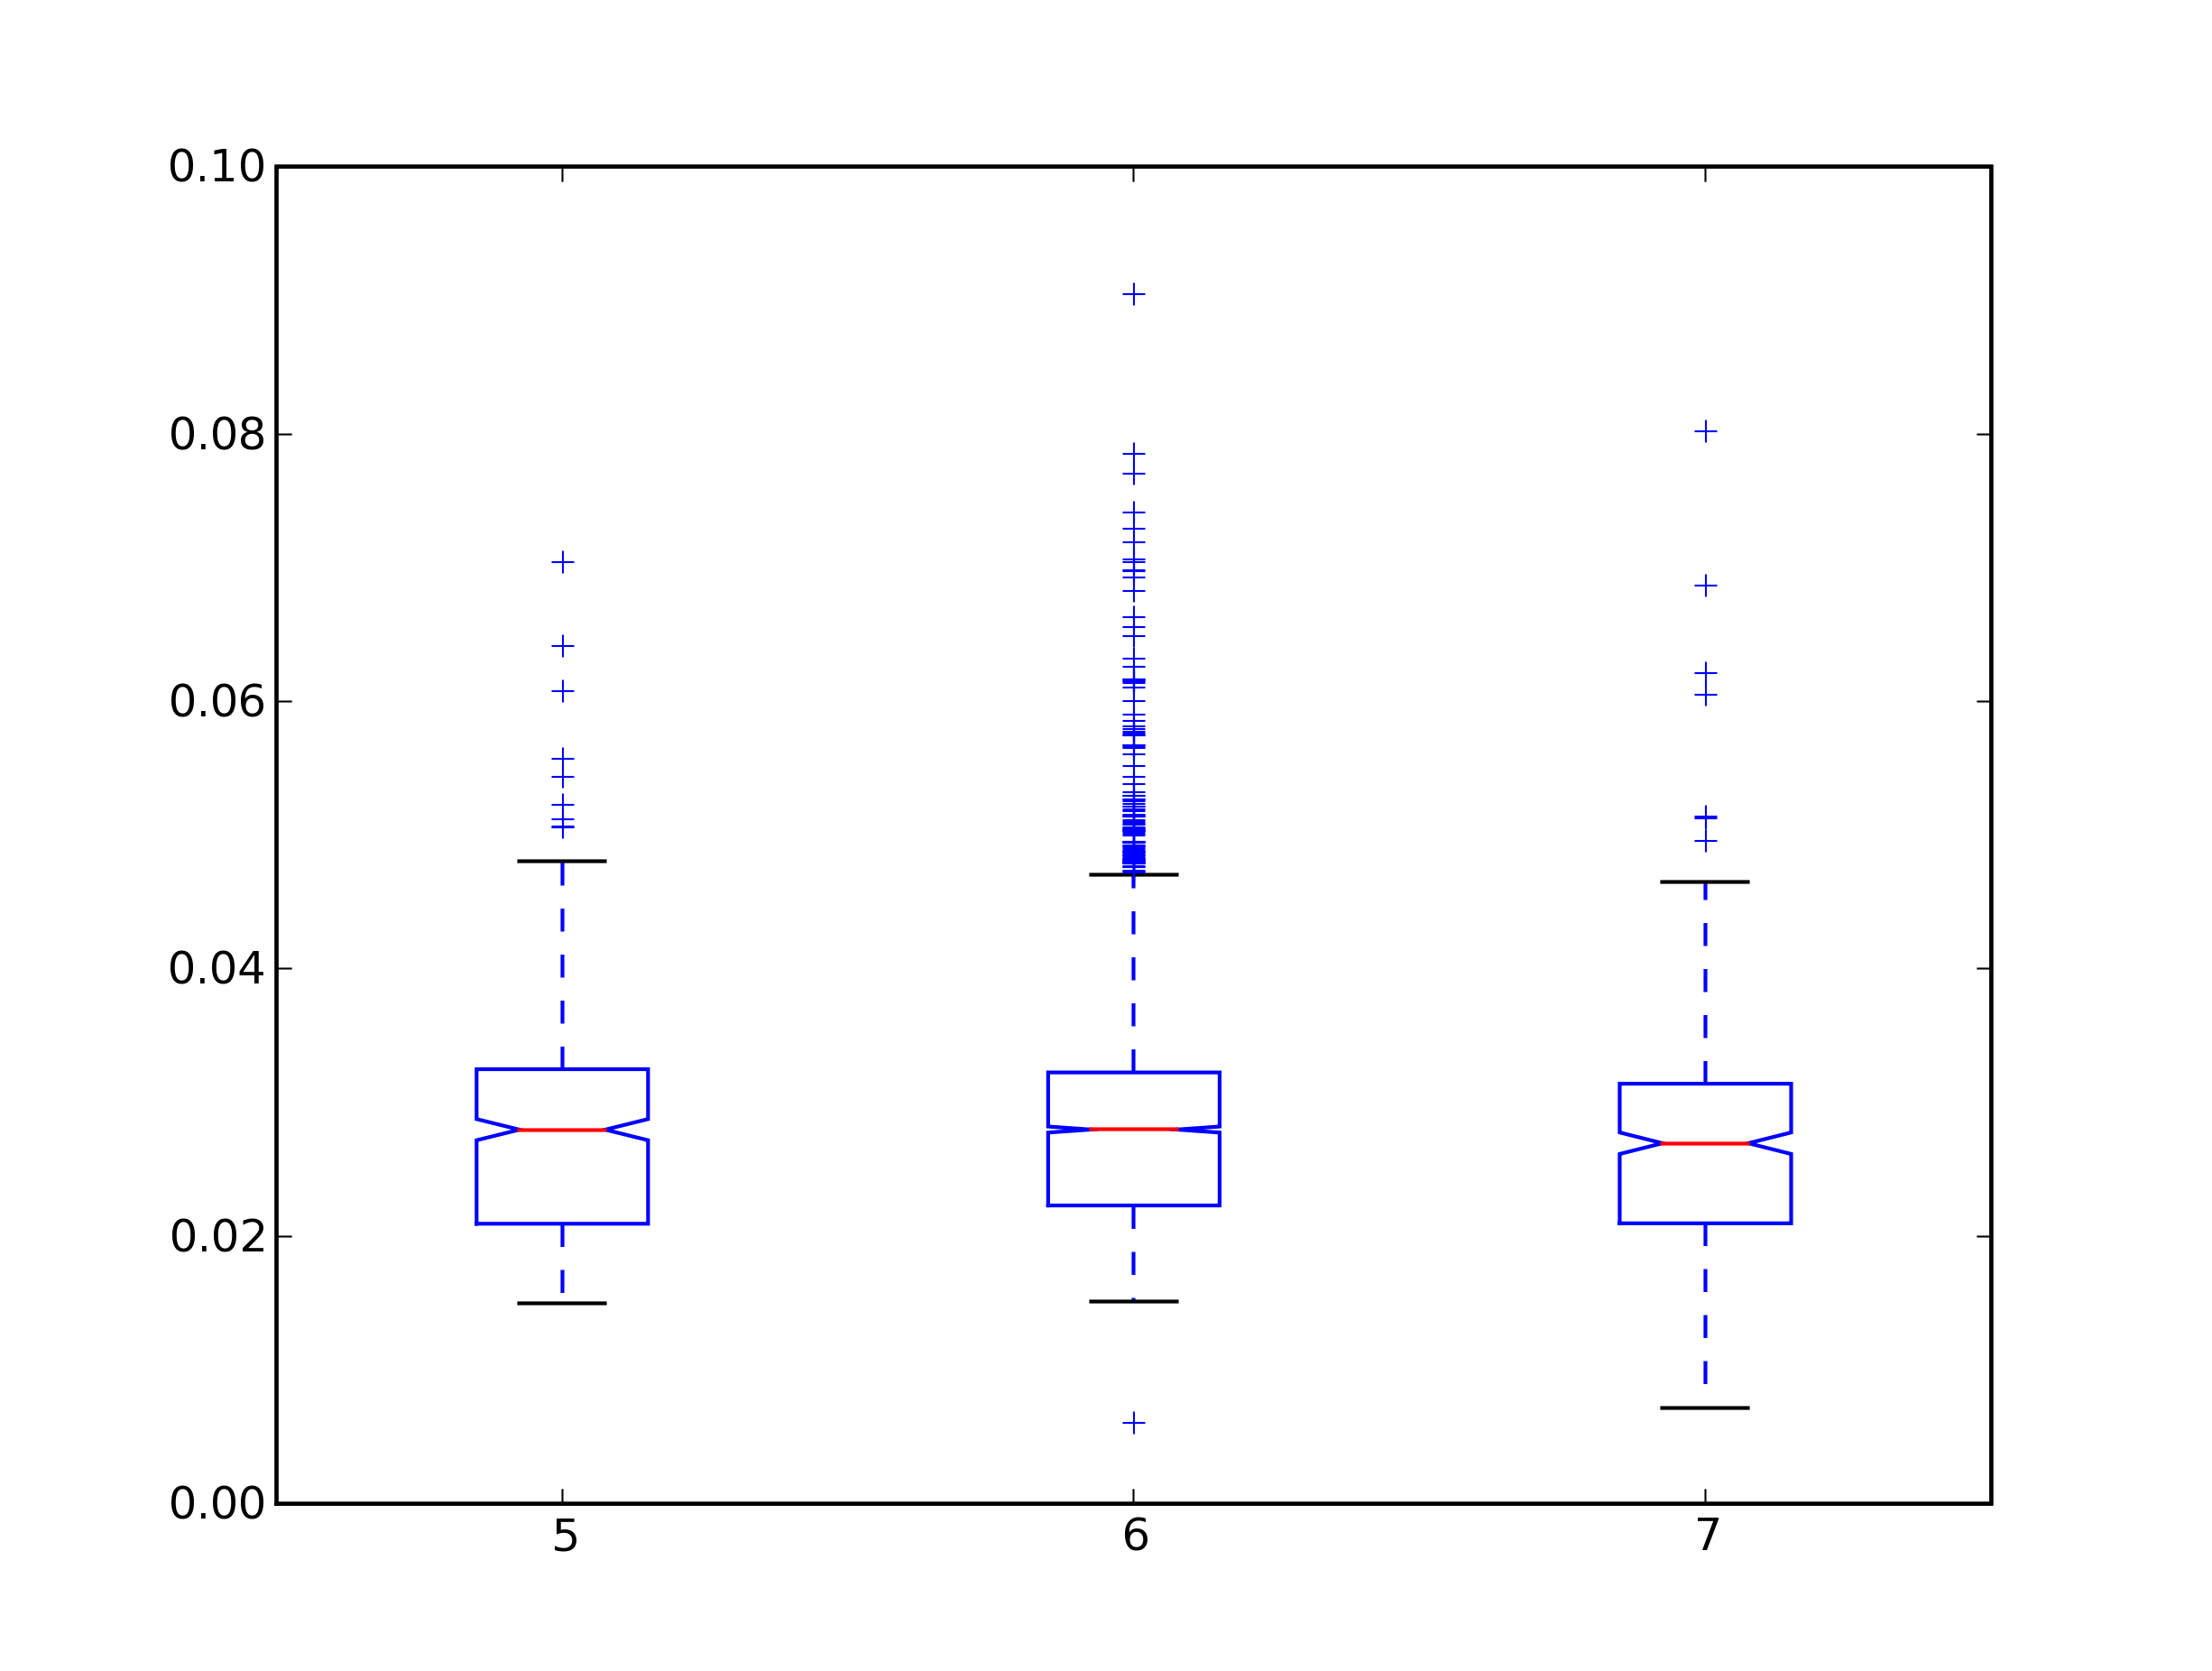
\includegraphics[width=.45\linewidth]{graph_iv_box.png}
}
\subfigure[Geodesic Sphere Topology]{
  \label{boxplot:geodesic}
  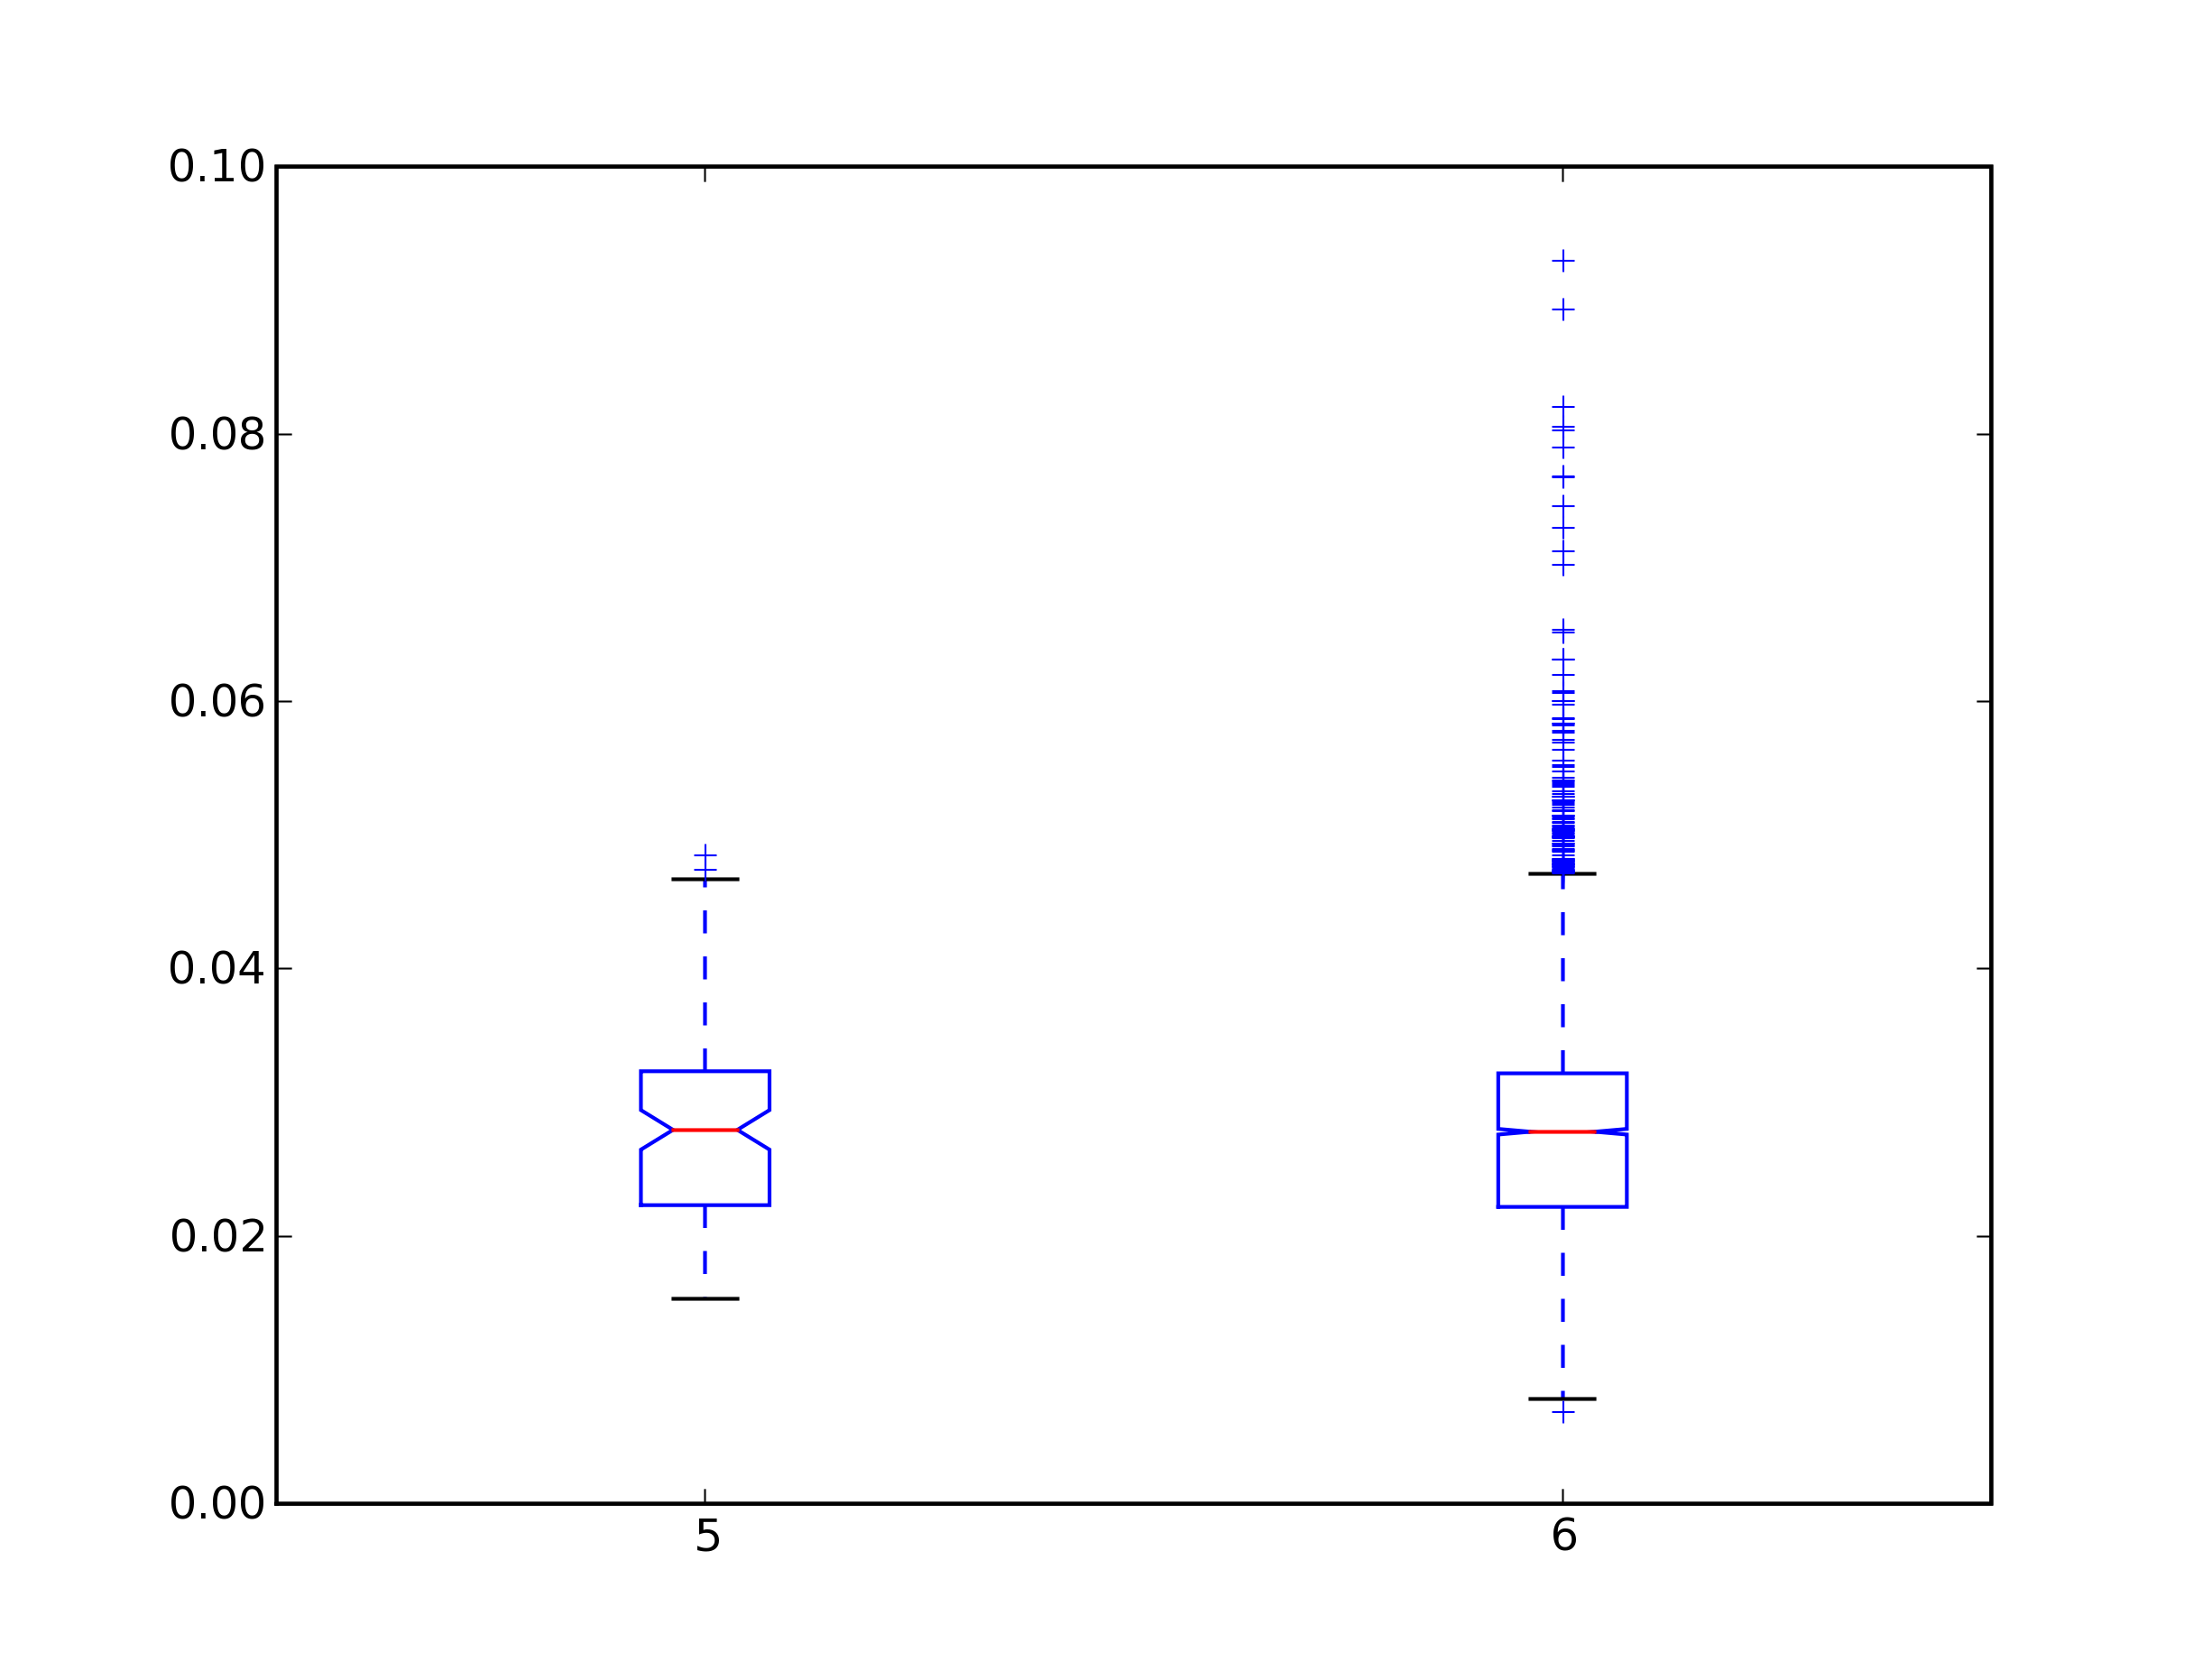
\includegraphics[width=.45\linewidth]{geodesic_iv_box.png}
}
\caption{This shows 4 box plots, each representing one group of neurons in a set
of SOMs trained with the same parameters.}
\end{figure}

Table \ref{meanvar1} shows the mean internal variance for each group for each
topology. Again we see that the internal variances seem to respond as expected
in the ``flat'' topologies, but not in the spherical topologies.  This is not
necessarily bad, as it may suggest that the spherical topologies are
effectively overcoming the edge problem.  The difference between these means
and their significance is presented in tables \ref{rlt}.  For the rook
topology table \ref{rlt:rook} shows that its three groups are significantly
different from each other. Results are similar for the hexagonal topology. For
the Spherical and Geodesic Topologies however there is no significant
different between in the groups.
%I suspect a better measure would be to use the minimum number of steps for a
%given nueron to reach every other neuron on the network.  This would vary
%significantly on the rook and hexagon topolgoies, but not very much in the
%spherical topologies.

\begin{table}[hbt]
\centering
\caption{Mean IV and Var(IV) grouped by a neurons degree for each topology}
\label{meanvar1}
\begin{tabular}{|c||c|c||c|c||c|c||c|c|}
\hline
\textbf{Degree} & \multicolumn{2}{c||}{\textbf{Geodesic}} &
\multicolumn{2}{c||}{\textbf{Spherical}} & \multicolumn{2}{c||}{\textbf{Hex}} &
\multicolumn{2}{c|}{\textbf{Rook}} \\
\hline
%& N & MeanIV & N & MeanIV & N & MeanIV & N & MeanIV \\
& N & Mean (Var) & N & Mean (Var) & N & Mean (Var) & N & Mean (Var) \\

\hline
2&&&&& 20& 0.1155 (0.0010)& 40& 0.1023 (0.0007)\\ 
3&&&&& 224& 0.1049 (0.0012)& 922& 0.0958 (0.0010)\\ 
4&&&&& 512& 0.1001 (0.0011)& 5227& 0.0877 (0.0010)\\ 
5& 115& 0.0876 (0.0013)& 563& 0.0875 (0.0010)& 209& 0.0935 (0.0011)&&\\ 
6& 6007& 0.0874 (0.0009)& 5124& 0.0880 (0.0010)& 5233& 0.0863 (0.0010)&&\\ 
7&&& 445& 0.0875 (0.0011)&&&&\\ 
%2&&&&& 20& 0.1109& 40& 0.1123\\ 
%3&&&&& 223& 0.1054& 918& 0.0997\\ 
%4&&&&& 507& 0.0980& 5138& 0.0875\\ 
%5& 115& 0.0898& 557& 0.0886& 208& 0.0921&&\\ 
%6& 5929& 0.0884& 5034& 0.0883& 5184& 0.0881&&\\ 
%7&&& 437& 0.0873&&&&\\ 
\hline
\end{tabular} \end{table}

%\subsection{Restate the Questions}
%\textbf{Objective}, Compare the internal variance of observations captured by a given
%neuron to that neuron's first-order neighborhood size.
%\textbf{Question}, Does the internal variance of a neuron decrease as its first-order
%neighborhood size, or degree, increases?


\begin{table}
\centering
\caption{These tables show the difference in means between each group of a
given topology and the significance of the difference,  delta (significance),
t=9999, *** = 99\%, ** = 95\%, * = 90\%}
\label{rlt}
  \subtable[Rook Topology]{
    \label{rlt:rook}
    \begin{tabular}{|c||c|c|c|}
    \hline
    &3&4\\\hline
    \hline
    2& 0.0065& \textbf{0.0147} ***\\\hline
    3& & \textbf{0.0082} ***\\\hline
  \end{tabular}
  }

  \subtable[Hexagonal Topology]{
    \label{rlt:hex}
    \begin{tabular}{|c||c|c|c|c|}
    \hline
    &3&4&5&6\\ \hline
    \hline
    2& 0.0106& \textbf{0.0154} **& \textbf{0.0220} ***& \textbf{0.0292} ***\\\hline
    3& & \textbf{0.0048} *& \textbf{0.0114} ***& \textbf{0.0186} ***\\\hline
    4& & & \textbf{0.0066} **& \textbf{0.0138} ***\\\hline
    5& & & & \textbf{0.0072} ***\\\hline
    \end{tabular}
  }

  \subtable[Spherical Topology]{
    \label{rlt:graph}
    \begin{tabular}{|c||c|c|}
    \hline
    &6&7\\ \hline
    \hline
    5& 0.0005& 0.0000\\\hline
    6& & 0.0005\\\hline

    \end{tabular}
  }

  \subtable[Geodesic Topology]{
    \label{rlt:geodesic}
    \begin{tabular}{|c||c|}
    \hline
    &6\\ \hline
    \hline
    5& 0.0001\\\hline
    \end{tabular}
  }
\end{table}

\section{next question}
This is the next section.  Here is TABLE \ref{rlt:all}.
  \begin{table}
  \centering
  \caption{These tables show the difference in means of the internal variance
between each topology}
  \label{rlt:all}
  \begin{tabular}{|c||c|c|c|c|}
  \hline
  \textbf{Topology}&Geodesic&Sphere&Hexagonal&Rook\\\hline
  \hline
  Geodesic&& 0.0005& \textbf{0.0010} *& \textbf{0.0015} ***\\\hline
  Sphere&& & 0.0005& \textbf{0.0011} *\\\hline
  Hexagonal&& & & 0.0005\\\hline
  Rook&& & & \\\hline
  \end{tabular}
  \end{table}

